A teszter elkészítése után a rendszer tesztelése következett.
A rendszer nem fektetett nagy hangsúlyt a pontossárga, viszont egy 
megközelítő értéket meg kell tudjon határozni.

\section{Ellenállás mérés}

Amennyiben az elkatrész egy ellenállás akkor meghatározza ennek az ellenállását.
Mivel az ADC-n levő konstans és változó zajok vannak és ezen alapszik 
az áramerősség mérése, így a mérések pontossága nem magas[\ref{fig:ResistorResults}], ami különösen csökken a mérés tartomány
végén, mivel a mérő ellenállás amit az áramerősség mérésére használ túl alacsony így
nem képes pontosan meghatározni az áramerősséget. Ezt egy nagyobb mérő ellenállással
lehetne korrigálni


\begin{table}[H]
    \begin{tabular}{|l|l|l|l|}
    \hline
    Sorszám & Névleges érték(Ohm) & Multiméterrel mért érték(Ohm) & Teszter által mért érték(Ohm) \\ \hline
    0       & 47             & 47                       & 52.5                     \\ \hline
    1       & 56             & 55.7                     & 59                       \\ \hline
    2       & 100            & 100.1                    & 107.4                    \\ \hline
    3       & 220            & 218                      & 242                      \\ \hline
    4       & 360            & 356                      & 398                      \\ \hline
    5       & 540            & 544                      & 606                      \\ \hline
    6       & 1000           & 980                      & 890                      \\ \hline
    7       & 2200           & 2198                     & 2301.7                   \\ \hline
    8       & 4700           & 4670                     & 4319.7                   \\ \hline
    9       & 10000          & 9680                     & 9237                     \\ \hline
    10      & 33000          & 32660                    & 28305.7                  \\ \hline
    11      & 62000          & 62000                    & 49590                    \\ \hline
    \end{tabular}
    \end{table}

    \begin{figure}[H]
        \centering
        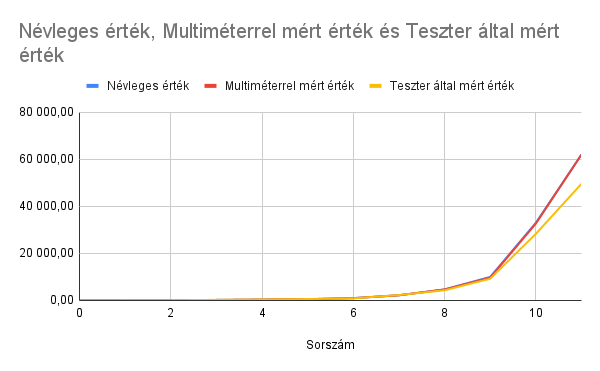
\includegraphics[scale=0.6]{images/results/resistorMesurement.png}
        \caption{Ellenállás mérés eredménye}
        \label{fig:ResistorResults}
    \end{figure}


\section{Kondenzátor}

Kondenzátor mérés estén az időt méri ameddig a kondenzátor feszültsége eléri a 
68\%-át a 3.3V-os forrásnak. Ezen esetben a mérés pontosabb, mivel
a zajok kevésbé befolyásolják így nem kell alacsony értékekből
számolni ami nagy hibához vezet. 50nF alatt nem biztos a mérés, 
mivel egyes alaktrészeket másnak is detektálhat, különösen ha 
hosszú vezetékek vannak használva. A grafikonon[\ref{fig:ResistorResults}]
látható, hogy a mérés jól megközelíti a névleges és dedikált mérőműszer
eredményeit.

\begin{table}[h]
    \begin{tabular}{|l|l|l|l|}
    \hline
    sorszám & Névleges érték & Mérőműszerrel mért érték & Mért érték \\ \hline
    1       & 60nF           & 59.62nF                  & 60nF       \\ \hline
    2       & 75nF           & 74.26                    & 75nF       \\ \hline
    3       & 100nF          & 98.26nF                  & 101nF      \\ \hline
    4       & 200nF          & 202nF                    & 203nF      \\ \hline
    5       & 300nF          & 300.3nF                  & 305nF      \\ \hline
    6       & 400nF          & 400nF                    & 406nF      \\ \hline
    7       & 500nF          & 498nF                    & 504nF      \\ \hline
    8       & 600nF          & 602nF                    & 610nF      \\ \hline
    9       & 700nF          & 701nF                    & 703nF      \\ \hline
    10      & 800nF          & 791.4nF                  & 800nF      \\ \hline
    11      & 900nF          & 889.7nF                  & 889nF      \\ \hline
    12      & 1uF            & 979nF                    & 1.059uF    \\ \hline
    13      & 2uF            & 1.97uF                   & 2.033uF    \\ \hline
    14      & 3uF            & 2.95uF                   & 3.05uF     \\ \hline
    15      & 4uF            & 3.96uF                   & 4.025uF    \\ \hline
    16      & 5uF            & 4.94uF                   & 5uF        \\ \hline
    17      & 6uF            & 5.935uF                  & 6.016uF    \\ \hline
    18      & 7uF            & 6.914uF                  & 6.95uF     \\ \hline
    19      & 8uF            & 7.946uF                  & 8.05uF     \\ \hline
    \end{tabular}
    \end{table}

    \begin{figure}[H]
        \centering
        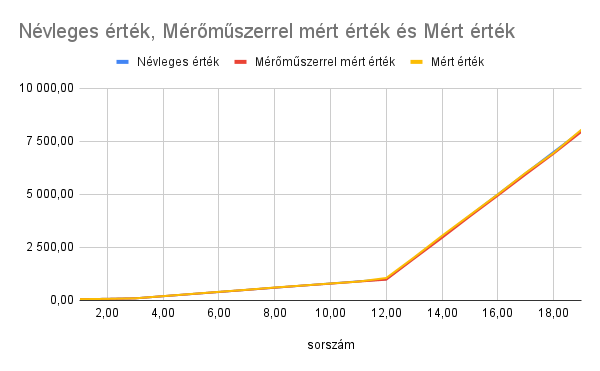
\includegraphics[scale=0.6]{images/results/CapacitorMeasurement.png}
        \caption{Kondenzátor mérés eredménye}
        \label{fig:CapacitorResults}
    \end{figure}

\section{Dióda}

A dióda mérés a diódán eső feszültséget méri miközben az egyik oldala
tápfeszültségen van és a kapcsoló ellenállások használatával.
A mérések során azt tapasztaltam, hogy a multiméter alacsonyabb
értékekett adott, míg a teszter nagyobbakat, viszont a LED-ek
tesztelése során világosabban villant fel. Így arra a következtetésre
jutottam, hogy a multiméter azt a feszültséget mérte ahol
minimálisan elkezdett a dióda vezetni és a teszter meg amikor
már teljesen nyitva van. A kék LED esetében a multiméter nem volt képes
megmérni a nyitó feszültséget, viszont ez 2.5 és 3.7V közt helyezkedhet el.

2 inverz diódát is képes megmérni, ebben az esetben azt adja vissza, hogy melyik
irányban mekkora a dióda nyitó feszültsége.

\begin{table}[H]
    \begin{tabular}{lll}
    Sorszám                 & Mérőműszerrel mért érték                  & Mért érték                \\ \hline
    \multicolumn{1}{|l|}{0} & \multicolumn{1}{l|}{0,54}                 & \multicolumn{1}{l|}{0,69} \\ \hline
    \multicolumn{1}{|l|}{1} & \multicolumn{1}{l|}{1,58}                 & \multicolumn{1}{l|}{1,8}  \\ \hline
    \multicolumn{1}{|l|}{2} & \multicolumn{1}{l|}{1.85}                 & \multicolumn{1}{l|}{1,96} \\ \hline
    \multicolumn{1}{|l|}{3} & \multicolumn{1}{l|}{1,78}                 & \multicolumn{1}{l|}{2,01} \\ \hline
    \multicolumn{1}{|l|}{4} & \multicolumn{1}{l|}{kék LED, nem mérhető} & \multicolumn{1}{l|}{2,83} \\ \hline
\end{tabular}
\end{table}

\section{Tranzisztor}

Ebben az esetben 

\section{Karakterisztika diagramm}

